\section{Sinais de Eletromiografia}
% ---

Sinais de EMG podem ser adquiridos por eletrodos posicionados na superfície da pele (eletrodo não invasivo) ou por agulhas introduzidas no tecido muscular (eletrodo invasivo). Sinais de EMG são compostos por potenciais de ação de fibras musculares organizadas em unidades funcionais chamadas de "unidades motoras" (MU - \emph{Motor Unit}) (DE LUCA \emph{et al}. 2006). Uma unidade motora é composta por um neurônio motor e as fibras musculares que ele inerva, e é a entidade fundamental que controla a ativação de músculos estriados (BUCHTAL and SCHMALBRUCH, 1980). A soma algébrica dos potenciais de ação de todas as fibras de uma unidade motora é chamada de "potencial de ação da unidade motora", ou em inglês, MUAP (\emph{Motor Unit Action Potential}) (ALMEIDA, 1997). A Figura \ref{fig_MUAP_comp} apresenta a composição de uma MUAP a partir da soma dos potenciais das fibras de uma unidade motora.

\begin{figure}[!htb]
	\caption{\label{fig_MUAP_comp}Soma de potenciais de ação das \emph{n} fibras de uma unidade motora, formando uma MUAP \emph{h(t)}.}
	\begin{center}
	    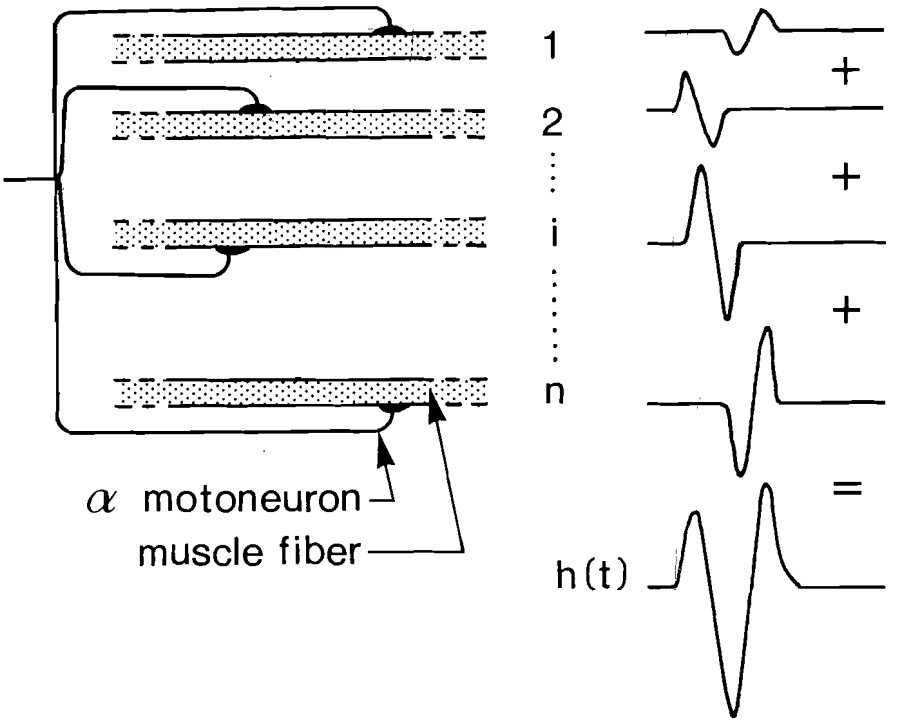
\includegraphics[width=0.75\linewidth]{./img/MUAP_oneMU.png}
	\end{center}
	\legend{Fonte: adaptado de BASMAJIAN \& DE LUCA, 1985}
\end{figure}

Dependendo do método utilizado para aquisição de EMG, é comum a captura da contribuição de mais de uma unidade motora no mesmo canal. A influência de uma unidade motora no sinal adquirido depende principalmente da distância das fibras musculares ao ponto de aquisição (HAMMARBERG and STERNAD, 2002). Sinais de EMG de longa duração são constituídos por sequências temporais de MUAPs, também conhecidas como MUAPTs (\emph{MUAP Trains}). A Figura \ref{fig_MUAP_trains} exemplifica MUAPTs de diferentes MUs que somam-se para formar um sinal de EMG de longa duração.

\begin{figure}[!htb]
	\caption{\label{fig_MUAP_trains}MUAPTs de diferentes MUs somam-se para compor o sinal adquirido por um canal de EMG.}
	\begin{center}
	    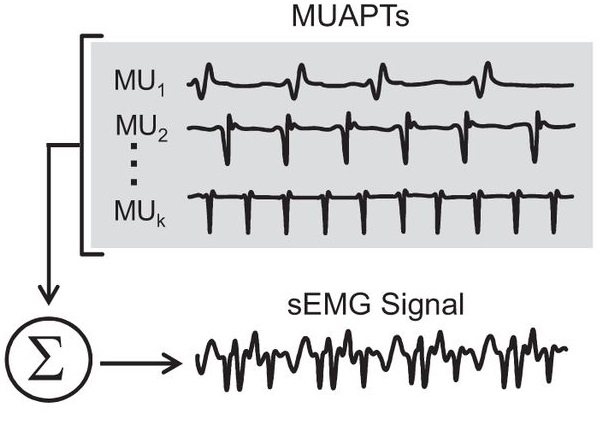
\includegraphics[width=0.75\linewidth]{./img/MUAP_trains.jpg}
	\end{center}
	\legend{Fonte: adaptado de KLINE \& DE LUCA, 2014}
\end{figure}

% ---
\section{Métodos de Segmentação}
% ---

Esta seção descreve os métodos de segmentação que foram utilizados como base teórica para os métodos desenvolvidos neste trabalho. Nota-se que nomes utilizados para variáveis e constantes (por exemplo, sinal a ser segmentado `$x$', \emph{threshold} `$T$', etc.) foram determinados pelo autor deste estudo, não necessariamente sendo estes utilizados nos métodos originais.

Para as definições dos métodos 3 e 4 (MTD3 e MTD4) são utilizados os termos BEP (\emph{beginning extraction point}, ponto inicial de um segmento) e EEP (\emph{ending extraction point}, ponto final de um segmento), também utilizados em (PATTICHIS \emph{et al}. 1995).
	
% ---
\subsection{Método 1 - método iterativo utilizando \emph{thresholding} para detecção de centros de segmentos de comprimento constante (MTD1)}
% ---

Este é o método iterativo de segmentação utilizado em (CHAUVET \emph{et al}. 2001). As definições da Tabela \ref{tab_mtd1params} serão utilizados para descrever este método.
\begin{table}[htb]
\IBGEtab{%
	\caption{Parâmetros utilizados para definir MTD1.}%
	\label{tab_mtd1params}
}{%
	\begin{tabular}{ccc}
	\toprule
	Nome & Descrição \\
	\midrule \midrule
	$x$ & Sinal a ser segmentado \\
	\midrule
	$L$ & Comprimento total do sinal a ser segmentado \\
	\midrule
	$l$ & Comprimento desejado para os segmentos \\
	\midrule
	$T_k$ & Valor de \emph{threshold} para a iteração $k$ \\
	\midrule
	$T_{lim}$ & Valor de limite inferior para o \emph{threshold} \\
	\midrule 
	$q$ & Fração de $T_{k-1}$ para determinação de $T_k$ \\
	\midrule 
	$N_{k}$ & Número total de candidatos para centros de segmentos identificados na iteração $k$ \\
	\midrule 
	$r_k$ & Razão entre número de candidatos identificados na iteração $k$ e o comprimento total do sinal \\
	\midrule 
	$r_{target}$ & Razão mínima esperada para $r_k$, utilizada para determinar o final do método \\
	\bottomrule
\end{tabular}%
}{%
}
\end{table}

Inicialmente, determina-se o valor de \emph{threshold} $T_0$ equivalente ao máximo absoluto do sinal a ser segmentado $x$ (Equação (\ref{eq:mtd1t0})). O valor $T_k$ é atualizado em cada iteração $k$ como sendo uma fração $q$ de $T_{k-1}$ (Equação (\ref{eq:mtd1tk})). No trabalho de (CHAUVET \emph{et al}. 2001), este valor $q$ foi empiricamente determinado em 90\%.

\begin{equation}
\label{eq:mtd1t0}
  T_0 = max(x)
\end{equation}

\begin{equation}
\label{eq:mtd1tk}
  T_k = q \times T_{k-1}
\end{equation}

Pontos do sinal acima do valor de $T_k$ são possíveis candidatos para centros de segmentos. Caso exista mais de um possível candidato em uma vizinhança bilateral de $l$ amostras do sinal, apenas o ponto de maior amplitude nesta vizinhança é considerado. Para determinar o final do método, avalia-se a razão $r_k$ entre a quantidade identificada de candidatos $N_{k}$ e o comprimento total do sinal $L$ (Equação (\ref{eq:mtd1rk})). Caso $r_k$ seja menor que um valor predeterminado $r_{target}$, calcula-se $T_{k+1}$ para realização da próxima iteração (Equação (\ref{eq:mtd1tk})). Caso $r_k$ seja maior ou igual ao valor predeterminado $r_{target}$, encerra-se o método e os segmentos são tomados como janelas de sinal de comprimento $l$, centradas nos candidatos identificados na última iteração.

\begin{equation}
\label{eq:mtd1rk}
  r_k = \frac{N_{k}}{L} 
\end{equation}

Adicionalmente, o estabelecimento de um valor limite mínimo para \emph{threshold} $T_{lim}$ garante que o método não entre em laço infinito e evita detecção de segmentos em trechos de baixa atividade muscular. Caso o valor de \emph{threshold} $T_k$ para a iteração atual seja inferior a $T_{lim}$, encerra-se o processo iterativo. O método de segmentação MTD1 é representado pelo fluxograma da Figura \ref{fig_mtd1flux}.

\begin{figure}[!htb]
	\caption{\label{fig_mtd1flux}Fluxograma representativo do MTD1.}
	\begin{center}
		\begin{tikzpicture}[node distance = 2cm, auto]
			% Place nodes
			\node [block] (init) {INÍCIO\\ \vspace{\onelineskip} $k = 0$\\$T_0 = max(x)$};
			\node [block, below = 1cm of init] (update) {$k++$\\$T_k = q \times T_{k-1}$};
			\node [decision, below = 1cm of update] (check_t) {$T_k < T_{lim}$?};
			\node [block, right = 2cm of check_t] (identify) {Identificar candidatos a centros de segmentos};
			\node [decision, right = 1cm of identify, text width = 8em] (decide) {$\frac{N_k}{L} >= r_{target}$?};
			\node [block, below = 1cm of check_t] (stop) {Segmentos de comprimento $l$ centrados nos candidatos identificados\\ \vspace{\onelineskip} FIM};
			
			% Draw edges
			\path [line] (init) -- (update);
			\path [line] (update) -- (check_t);
			\path [line] (check_t) -- node [near start] {SIM} (stop);
			\path [line] (check_t) -- node [near start] {NÃO} (identify);
			\path [line] (identify) -- (decide);
			\path [line] (decide) |- node [near start] {SIM} (stop);
			\path [line] (decide) |- node [near start] {NÃO} (update);
			
		\end{tikzpicture}
	\end{center}
\end{figure}

% ---
\subsection{Método 2 - método não iterativo utilizando \emph{thresholding} para detecção de centros de segmentos de comprimento constante (MTD2)}
% ---

Este é o método de segmentação utilizado em (KATSIS \emph{et al}. 2006), que será descrito pelas definições da Tabela \ref{tab:mtd2params}. Primeiramente, seleciona-se entre dois métodos de cálculo de \emph{threshold} $T$: ou utiliza-se $T$ como múltiplo da média aritmética do sinal $x$; ou $T$ é uma fração do valor máximo do sinal $x$. O trabalho de (KATSIS \emph{et al}. 2006) utiliza a relação do fluxograma da Figura \ref{fig_mtd2flux} para o cálculo de \emph{threshold} $T$.

\begin{table}[htb]
\IBGEtab{%
	\caption{Parâmetros utilizados para definir MTD2.}%
	\label{tab:mtd2params}
}{%
	\begin{tabular}{ccc}
	\toprule
	Nome & Descrição \\
	\midrule \midrule
	$x$ & Sinal a ser segmentado \\
	\midrule
	$L$ & Comprimento total do sinal a ser segmentado \\
	\midrule
	$l$ & Comprimento desejado para os segmentos \\
	\midrule
	$T$ & Valor de \emph{threshold} \\
	\midrule
	$A$ & Coeficiente utilizado para decisão de método de cálculo de $T$ \\
	\midrule
	$B$ & Múltiplo da média aritmética do sinal $x$ para obtenção de $T$ \\
	\midrule
	$C$ & Fração do valor máximo do sinal $x$ para cálculo de $T$ \\
	\bottomrule
\end{tabular}%
}{%
}
\end{table}

\begin{figure}[!htb]
	\caption{\label{fig_mtd2flux} Fluxograma representativo do MTD2.}
	\begin{center}
		\begin{tikzpicture}[node distance = 2cm, auto]
			% Place nodes
			\node [block] (init) {INÍCIO};
			\node [decision, below = 1cm of init,text width=10em] (decide) {$max(x) > \frac{A}{L}\sum_{i=1}^{L}|x_i|$?};
			\node [block, below left = 1cm and 1cm of decide] (case 1) {$T = \frac{B}{L}\sum_{i=1}^{L}|x_i|$};
			\node [block, below right = 1cm and 1cm of decide] (case 2) {$T = \frac{max(x)}{C}$};
			\node [block, below = 3cm of decide] (identify) {Identificar centros de segmentos};
			\node [block, below = 1cm of identify] (stop) {Segmentos de comprimento $l$ nos centros identificados\\ \vspace{\onelineskip} FIM};
			
			% Draw edges
			\path [line] (init) -- (decide);
			\path [line] (decide) -| node [near start] {SIM} (case 1);
			\path [line] (decide) -| node [near start] {NÃO} (case 2);
			\path [line] (case 1) -| (identify);
			\path [line] (case 2) -| (identify);
			\path [line] (identify) -- (stop);
		\end{tikzpicture}
	\end{center}
\end{figure}

De forma similar ao MTD1, os pontos do sinal que tiverem valor acima de $T$ são considerados possíveis candidatos para centros de segmentos. Para os possíveis candidatos que estiverem afastados de uma distância inferior a $l$, apenas o candidato de maior amplitude é considerado. Em (KATSIS \emph{et al}. 2006) utilizou-se coeficientes $A$, $B$ e $C$ respectivamente de 30, 5 e 5, com comprimento $l$ de 121 amostras.

% ---
\subsection{Método 3 - método com janela deslizante para detecção de BEP e EEP de segmentos utilizando variação total (MTD3)}
% ---

	Este é o método de segmentação utilizado em (GUT and MOSCHYTZ, 2000). As definições da Tabela \ref{tab:mtd3params} serão utilizados para descrever este método.
	
\begin{table}[htb]
\IBGEtab{%
	\caption{Parâmetros utilizados para definir MTD3.}%
	\label{tab:mtd3params}
}{%
	\begin{tabular}{ccc}
	\toprule
	Nome & Descrição \\
	\midrule \midrule
	$x$ & Sinal a ser segmentado \\
	\midrule
	$W$ & Comprimento da janela deslizante utilizada pelo método \\
	\midrule
	$w_0$ & Número da amostra mais a esquerda da janela. Determina a posição instantânea da janela \\
	\midrule
	$\beta$ & Declividade média do sinal $x$ contido na janela deslizante \\
	\midrule
	$B$ & Valor limite para declividade média que determina um BEP\\
	\midrule
	$\gamma$ & Variação total do sinal $x$ contido na janela deslizante \\
	\midrule
	$C$ & Valor limite para variação total que determina um EEP\\
	\bottomrule
\end{tabular}%
}{%
}
\end{table}

Uma janela deslizante de comprimento $W$ percorre o sinal da esquerda para a direita. Caso a declividade média $\beta$ do trecho de sinal contido pela janela, calculado pela Equação (\ref{eq:decMedia}), exceda um limite $B$, o ponto mais à esquerda da janela $w_0$ determina a BEP de um segmento.

\begin{equation}
\label{eq:decMedia}
	\beta = \frac{1}{W}\sum_{i=w_0+1}^{W}(x_i - x_{i-1})
\end{equation}

O EEP do correspondente segmento é então obtido como o ponto mais à direita da janela ($w_0 + W - 1$) quando a variação total $\gamma$, dado pela Equação (\ref{eq:varTotal}), do trecho de sinal contido pela janela for menor que um limite $C$.

\begin{equation}
\label{eq:varTotal}
	\gamma = \sum_{i=w_0+1}^{W}(x_i - x_{i-1})
\end{equation}

O MTD3 pode ser representado pelo fluxograma da Figura \ref{fig_mtd3flux}.

\begin{figure}[!htb]
	\caption{\label{fig_mtd3flux} Fluxograma representativo do MTD3.}
	\begin{center}
		\begin{tikzpicture}[node distance = 2cm, auto]
			% Place nodes
			\node [block] (init) {INÍCIO \\ \vspace{\onelineskip} $w_0 = 0$ \\ \vspace{\onelineskip} Janela de comprimento $W$, iniciando em $w_0$};
			\node [decision, below = 1cm of init, text width = 9em] (final_detect) {$w_0 \gets w_0 + 1$ \\ \vspace{\onelineskip} $w_0 > (L - W + 1)?$};
			\node [block, left = 1cm of init] (stop) {Segmentos formados pelos BEPs e EEPs identificados \\ \vspace{\onelineskip} FIM};
			\node [block, left = 2cm of final_detect, text width = 13em] (beta) {$\beta = \frac{1}{W-1}\sum_{i=w_0}^{w_0+W-1}(x_{i+1} - x_i)$};
			\node [decision, below = 1cm of beta] (BEP_decide) {$\beta > B$?};
			\node [block, below = 1cm of BEP_decide] (BEP_detected) {$w_0$ é BEP};
			\node [decision, below = 2cm of BEP_detected, text width = 9em] (w0pp) {$w_0 \gets w_0 + 1$ \\ \vspace{\onelineskip} $w_0 > (L - W + 1)?$};
			\node [block, right = 2cm of w0pp, text width = 13em] (gamma) {$\gamma = \sum_{i=w_0}^{w_0+W-1}(x_{i+1} - x_i)$};
			\node [decision, above = 1cm of gamma] (EEP_decide) {$\gamma < C$?};
			\node [block, above = 1cm of EEP_decide] (EEP_detected) {$(w_0 + W - 1)$ é EEP};
			\node [block, left = 1cm of stop] (discard) {Descartar último BEP};
			
			% Draw edges
			\path [line] (init) -- (final_detect);
			\path [line] (final_detect) -- node [near start] {SIM} (stop);
			\path [line] (final_detect) -- node [near start] {NÃO} (beta);
			\path [line] (beta) -- (BEP_decide);
			\path [line] (BEP_decide) -| node [near start] {NÃO} (final_detect);
			\path [line] (BEP_decide) -- node [near start] {SIM} (BEP_detected);
			\path [line] (BEP_detected) -- (w0pp);
			\path [line] (w0pp) -- node [near start] {NÃO} (gamma);
			\path [line] (gamma) -- (EEP_decide);
			\path [line] (EEP_decide) -- node [near start] {SIM} (EEP_detected);
			\path [line] (EEP_decide) -| node [near start] {NÃO} (w0pp);
			\path [line] (EEP_detected) -- (final_detect);
			\path [line] (w0pp) -| node [near start] {SIM}(discard);
			\path [line] (discard) -- (stop);
			
		\end{tikzpicture}
	\end{center}
\end{figure}

% ---
\subsection{Método 4 - método com janela deslizante para detecção de BEP e EEP de segmentos utilizando \emph{thresholding} (MTD4)}
% ---

Este é o método de segmentação utilizado em (PACHITTIS \emph{et al}. 1995). As definições da Tabela \ref{tab:mtd4params} serão utilizados para descrever este método.

\begin{table}[htb]
\IBGEtab{%
	\caption{Parâmetros utilizados para definir MTD4.}%
	\label{tab:mtd4params}
}{%
	\begin{tabular}{ccc}
	\toprule
	Nome & Descrição \\
	\midrule \midrule
	$x$ & Sinal a ser segmentado \\
	\midrule
	$L$ & Comprimento total do sinal $x$ \\
	\midrule
	$W$ & Comprimento da janela deslizante utilizada pelo método \\
	\midrule
	$T$ & Valor de \emph{threshold} \\
	\bottomrule
\end{tabular}%
}{%
}
\end{table}

Uma janela deslizante de comprimento $W$ com início em $w_0$ percorre o sinal da esquerda para a direita. Os BEPs dos segmentos são pontos $w_0$ tais que o valor máximo do sinal contido pela janela permanece abaixo do valor de \emph{threshold} $T$. Para sequências de pontos consecutivos que atendam esta especificação, seleciona-se o último ponto (ponto mais à direita). As EEPs são identificadas de forma similar, sendo os primeiros pontos $w_0 + W - 1$ após as BEPs nos quais o sinal contido pela janela permanece abaixo do valor de \emph{threshold} $T$.

No trabalho de (PACHITTIS \emph{et al}. 1995), utilizou-se janelas de comprimento $W$ correspondente a 3 $ms$ de aquisição e \emph{threshold} $T$ de $\pm$ 40 $\mu V$ (o sinal de EMG segmentado não era retificado). O fluxograma da Figura \ref{fig_mtd4flux} representa o MTD4.

\begin{figure}[!htb]
	\caption{\label{fig_mtd4flux} Fluxograma representativo do MTD4.}
	\begin{center}
		\begin{tikzpicture}[node distance = 2cm, auto]
			% Place nodes
			\node [block] (init) {INÍCIO \\ \vspace{\onelineskip} $w_0 = 0$ \\ \vspace{\onelineskip} Janela de comprimento $W$, iniciando em $w_0$};
			\node [decision, below = 1cm of init, text width = 8em] (beg_detect) {$w_0 \gets w_0 +1$ \\ \vspace{\onelineskip} $w_0 > L-W+1$?};
			\node [decision, below left = 1cm and 3cm of beg_detect, text width = 10em] (threshBEP) {Máximo do sinal contido na janela $< T$?};
			\node [block, below = 1cm of threshBEP] (BEP_detected) {$w_0$ é BEP};
			\node [decision, below = 2cm of BEP_detected, text width = 8em] (w0pp) {$w_0 \gets w_0 +1$ \\ \vspace{\onelineskip} $w_0 > L-W+1$?};
			\node [decision, above right = 1cm and 3cm of w0pp, text width = 10em] (threshEEP) {Máximo do sinal contido na janela $< T$?};
			\node [block, above = 1cm of threshEEP] (EEP_detected) {$w_0+W-1$ é EEP};
			\node [block, left = 1cm of init] (stop) {Segmentos formados pelos BEPs e EEPs identificados \\ \vspace{\onelineskip} FIM};
			\node [block, left = 1cm of stop] (discard) {Descartar último BEP};
			
			% Draw edges
			\path [line] (init) -- (beg_detect);
			\path [line] (beg_detect) -| node [near start] {NÃO} (threshBEP);
			\path [line] (threshBEP) -| node [near start] {SIM} (beg_detect);
			\path [line] (threshBEP) -- node [near start] {NÃO} (BEP_detected);
			\path [line] (BEP_detected) -- (w0pp);
			\path [line] (w0pp) -| node [near start] {NÃO} (threshEEP);
			\path [line] (w0pp) -| node [near start] {SIM} (discard);
			\path [line] (threshEEP) -| node [near start] {NÃO} (w0pp);
			\path [line] (threshEEP) -- node [near start] {SIM} (EEP_detected);
			\path [line] (EEP_detected) -- (beg_detect);
			\path [line] (discard) -- (stop);
			\path [line] (beg_detect) -- node [near start] {SIM} (stop);
			
		\end{tikzpicture}
	\end{center}
\end{figure}

% ---
\section{Base de Dados Utilizadas}
% ---
% ---
\subsection{Base de Dados Ninapro}
% ---
% ---
\subsection{Base de Dados do IEE}
% ---